\documentclass[11pt, letterpaper]{memoir}
\usepackage{HomeworkStyle}
\geometry{margin=1in}



\begin{document}

	\begin{center}
		{\large Quiz 4.2 -- Phase Boundaries}
	\end{center}
	{\large Name: \rule[-1mm]{4in}{.1pt} 
		
\noindent\hspace{-2.5em}
\begin{minipage}{0.65\linewidth}
	~ ~ ~ ~ Use the phase diagram at right to answer the following questions:
	
	\noindent
	\begin{itemize}
		\item Estimate the slopes of the A-B and the D-B transition lines (These should technically be curves, but the curvature between solid phases is usually small)
		
		\vspace{3em}
		\item If $\Delta H_{A-B}=2.5\dfrac{kJ}{mol}$ at $150.0~K$, find $\Delta V_{m,A-B}$
		
		\vspace{5em}
		\item If $\Delta V_{m,D-B}=2.3\dfrac{mm^3}{mol}$ at $200.0~K$, find $\Delta H_{D-B}$
	\end{itemize}
\end{minipage}~
\begin{minipage}{0.45\linewidth}
	\includegraphics[width=\textwidth]{Phase_Diagram2}
\end{minipage}

\vspace{5em}\noindent
Gasoline readily evaporates if it spills onto the ground. For gasoline, $\Delta H_{vap}=39.1\dfrac{kJ}{mol}$, and gasoline has a normal boiling temperature of $333~K$. What is the vapor pressure of gasoline at $20^\circ C$?

\vspace{5em}\noindent
You measure the vapor pressure of an unknown substance at two temperatures. At $260.0~K$ the vapor pressure is $13.5~torr$, and at $310.0~K$ the vapor pressure is $1240~torr$. Use these data to estimate $\Delta H_{vap}$ for this substance.

\vspace{5em}\noindent
Use today's barometric pressure to estimate the actual boiling temperature of water today in Cedar City, Utah.

\newpage
\pagestyle{empty}
\addtocounter{page}{-1}
\section*{\emph{Sonnet 18: Shall I compare thee to a summer’s day?}}
\paragraph{By William Shakespeare}~
\begin{verse}
	Shall I compare thee to a summer’s day?\\
	Thou art more lovely and more temperate:\\
	Rough winds do shake the darling buds of May,\\
	And summer’s lease hath all too short a date;\\
	Sometime too hot the eye of heaven shines,\\
	And often is his gold complexion dimm'd;\\
	And every fair from fair sometime declines,\\
	By chance or nature’s changing course untrimm'd;\\
	But thy eternal summer shall not fade,\\
	Nor lose possession of that fair thou ow’st;\\
	Nor shall death brag thou wander’st in his shade,\\
	When in eternal lines to time thou grow’st:\\
	\hspace{0.5em} So long as men can breathe or eyes can see,\\
	\hspace{0.5em} So long lives this, and this gives life to thee.
\end{verse}
\end{document}
